\documentclass[border=12pt]{standalone}
\usepackage{tikz}
\usetikzlibrary{shapes.geometric, arrows.meta, positioning, calc, fit, backgrounds}
\usepackage{fontspec}
\usepackage{amsmath,amssymb}
\setmainfont{DejaVu Sans}

\begin{document}
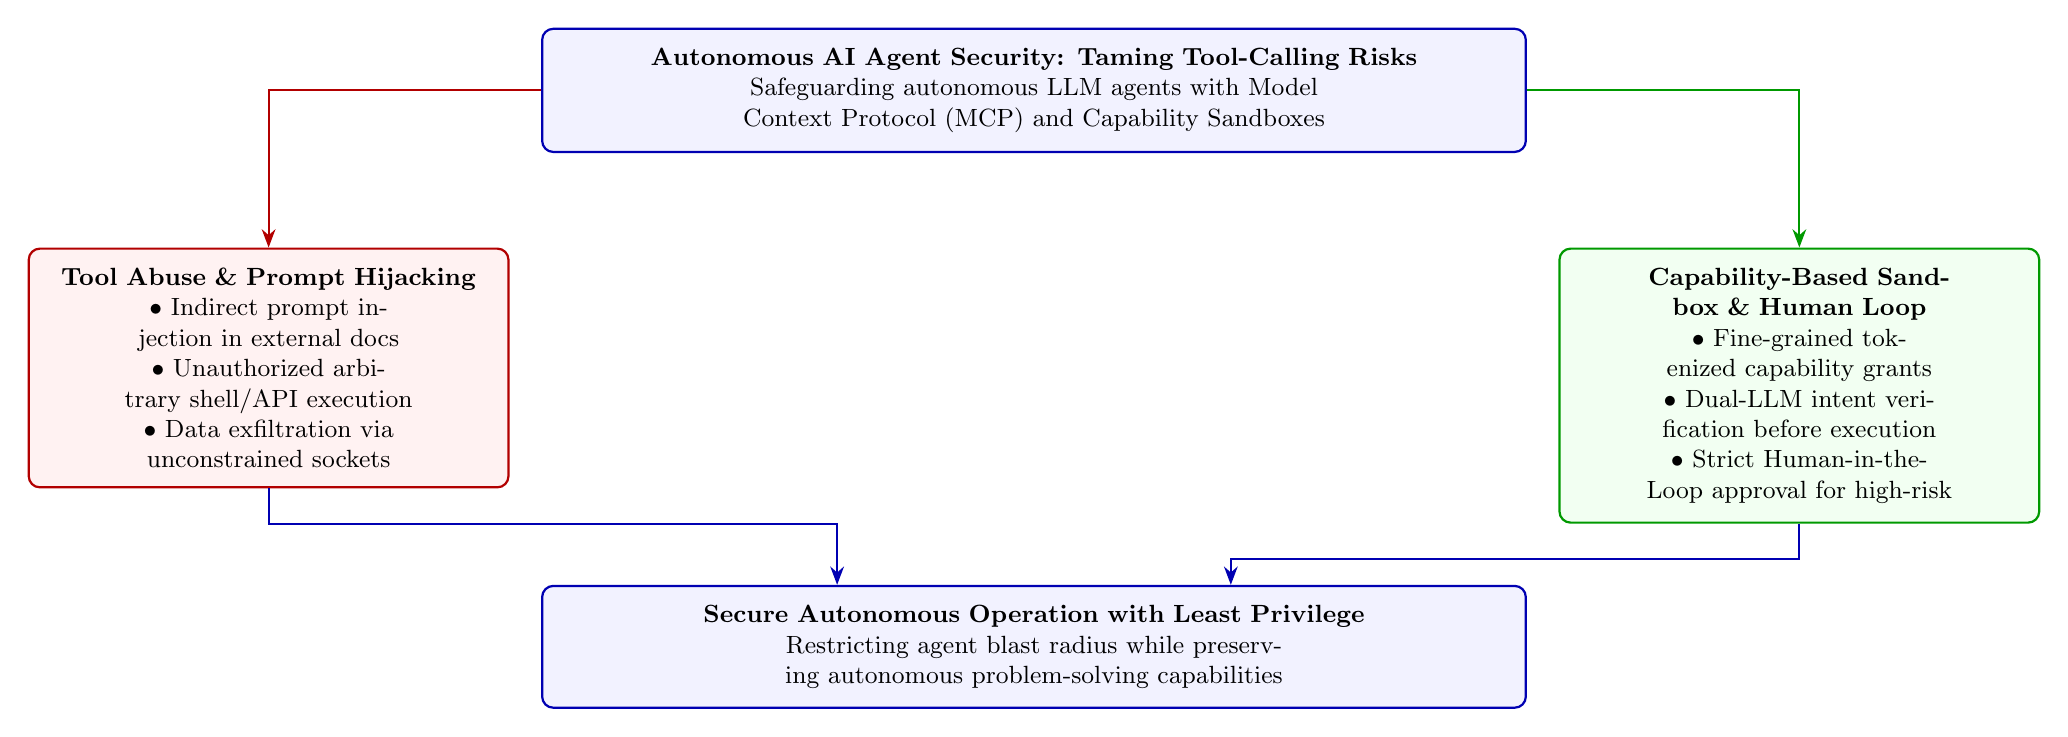
\begin{tikzpicture}[
    font=\small,
    >=Stealth,
    node distance=1.2cm,
    block/.style={rectangle, draw=blue!70!black, fill=blue!5, rounded corners=4pt, thick, align=center, inner sep=7pt},
    alertblock/.style={rectangle, draw=red!70!black, fill=red!5, rounded corners=4pt, thick, align=center, inner sep=7pt},
    greenblock/.style={rectangle, draw=green!60!black, fill=green!5, rounded corners=4pt, thick, align=center, inner sep=7pt},
    amberblock/.style={rectangle, draw=orange!80!black, fill=orange!5, rounded corners=4pt, thick, align=center, inner sep=7pt}
]

\node[block, text width=12cm] (top) {\textbf{Autonomous AI Agent Security: Taming Tool-Calling Risks}\\Safeguarding autonomous LLM agents with Model Context Protocol (MCP) and Capability Sandboxes};

\node[alertblock, below left=1.2cm and 0.4cm of top, text width=5.6cm] (agent_threat) {\textbf{Tool Abuse \& Prompt Hijacking}\\$\bullet$ Indirect prompt injection in external docs\\$\bullet$ Unauthorized arbitrary shell/API execution\\$\bullet$ Data exfiltration via unconstrained sockets};

\node[greenblock, below right=1.2cm and 0.4cm of top, text width=5.6cm] (agent_defense) {\textbf{Capability-Based Sandbox \& Human Loop}\\$\bullet$ Fine-grained tokenized capability grants\\$\bullet$ Dual-LLM intent verification before execution\\$\bullet$ Strict Human-in-the-Loop approval for high-risk};

\node[block, below=1.0cm of $(agent_threat.south)!0.5!(agent_defense.south)$, text width=12cm] (bottom) {\textbf{Secure Autonomous Operation with Least Privilege}\\Restricting agent blast radius while preserving autonomous problem-solving capabilities};

\draw[->, thick, red!70!black] (top) -| (agent_threat);
\draw[->, thick, green!60!black] (top) -| (agent_defense);
\draw[->, thick, blue!70!black] (agent_threat.south) -- ++(0,-0.45) -| ([xshift=-2.5cm]bottom.north);
\draw[->, thick, blue!70!black] (agent_defense.south) -- ++(0,-0.45) -| ([xshift=2.5cm]bottom.north);

\end{tikzpicture}
\end{document}
